\documentclass{beamer}

\pdfmapfile{+sansmathaccent.map}


\mode<presentation>
{
  \usetheme{Warsaw} % or try Darmstadt, Madrid, Warsaw, Rochester, CambridgeUS, ...
  \usecolortheme{seahorse} % or try seahorse, beaver, crane, wolverine, ...
  \usefonttheme{serif}  % or try serif, structurebold, ...
  \setbeamertemplate{navigation symbols}{}
  \setbeamertemplate{caption}[numbered]
} 


%%%%%%%%%%%%%%%%%%%%%%%%%%%%
% itemize settings

\definecolor{mypink}{RGB}{255, 150, 150}
\definecolor{myblue}{RGB}{150, 150, 255}
\definecolor{mygray}{gray}{0.8}

\setbeamertemplate{itemize items}[default]

\setbeamertemplate{itemize item}{\color{mypink}$\blacksquare$}
\setbeamertemplate{itemize subitem}{\color{myblue}$\blacktriangleright$}
\setbeamertemplate{itemize subsubitem}{\color{mygray}$\blacksquare$}

%%%%%%%%%%%%%%%%%%%%%%%%%%%%
% block settings

\setbeamercolor{block title}{bg=red!30,fg=black}


%%%%%%%%%%%%%%%%%%%%%%%%%%%%
% URL settings
\hypersetup{
    colorlinks=true,
    linkcolor=blue,
    filecolor=blue,      
    urlcolor=blue,
}

%%%%%%%%%%%%%%%%%%%%%%%%%%

\renewcommand{\familydefault}{\rmdefault}

\usepackage{amsmath}
\usepackage{mathtools}

\DeclareMathOperator*{\argmin}{arg\,min}

\usepackage{subcaption}




%%%%%%%%%%%%%%%%%%%%%%%%%%%%
% code settings

\usepackage{listings}
\usepackage{color}
\definecolor{mygreen}{rgb}{0,0.6,0}
\definecolor{mygray}{rgb}{0.5,0.5,0.5}
\definecolor{mymauve}{rgb}{0.58,0,0.82}
\lstset{ 
  backgroundcolor=\color{white},   % choose the background color; you must add \usepackage{color} or \usepackage{xcolor}; should come as last argument
  basicstyle=\footnotesize,        % the size of the fonts that are used for the code
  breakatwhitespace=false,         % sets if automatic breaks should only happen at whitespace
  breaklines=true,                 % sets automatic line breaking
  captionpos=b,                    % sets the caption-position to bottom
  commentstyle=\color{mygreen},    % comment style
  deletekeywords={...},            % if you want to delete keywords from the given language
  escapeinside={\%*}{*)},          % if you want to add LaTeX within your code
  extendedchars=true,              % lets you use non-ASCII characters; for 8-bits encodings only, does not work with UTF-8
  firstnumber=0000,                % start line enumeration with line 0000
  frame=single,	                   % adds a frame around the code
  keepspaces=true,                 % keeps spaces in text, useful for keeping indentation of code (possibly needs columns=flexible)
  keywordstyle=\color{blue},       % keyword style
  language=Octave,                 % the language of the code
  morekeywords={*,...},            % if you want to add more keywords to the set
  numbers=left,                    % where to put the line-numbers; possible values are (none, left, right)
  numbersep=5pt,                   % how far the line-numbers are from the code
  numberstyle=\tiny\color{mygray}, % the style that is used for the line-numbers
  rulecolor=\color{black},         % if not set, the frame-color may be changed on line-breaks within not-black text (e.g. comments (green here))
  showspaces=false,                % show spaces everywhere adding particular underscores; it overrides 'showstringspaces'
  showstringspaces=false,          % underline spaces within strings only
  showtabs=false,                  % show tabs within strings adding particular underscores
  stepnumber=2,                    % the step between two line-numbers. If it's 1, each line will be numbered
  stringstyle=\color{mymauve},     % string literal style
  tabsize=2,	                   % sets default tabsize to 2 spaces
  title=\lstname                   % show the filename of files included with \lstinputlisting; also try caption instead of title
}

%%%%%%%%%%%%%%%%%%%%%%%%%%%%
% tikz settings

\usepackage{tikz}
\tikzset{every picture/.style={line width=0.75pt}}


\title{Error dynamics and control of systems with constraints}
\subtitle{Contact-aware Control, Lecture 6}
\author{by Sergei Savin}
\centering
\date{Fall 2020}



\begin{document}
\maketitle


\begin{frame}{Content}

\begin{itemize}
\item Trajectory tracking; desired trajectory
\item Desired trajectory and constraints
\item Error dynamics
\begin{itemize}
\item Definition
\item Design
\item Computed torque controller
\item Feedback and feedforward
\end{itemize}
\item Control and constraints
\begin{itemize}
\item Calculating control input expressing reaction forces out
\item Calculating control input, accelerations and reaction forces simultaneously
\item Feasibility conditions
\end{itemize}
\item Algebra recap
\begin{itemize}
\item Fundamental subspaces
\item Projectors
\end{itemize}
\item Read more
\item Homework
\end{itemize}

\end{frame}



\begin{frame}{Trajectory tracking; desired trajectory}
% \framesubtitle{O}
\begin{flushleft}

Trajectory tracking is a control problem that says:

\begin{block}{Trajectory tracking}
Find such \emph{control law} $\bo{u} = \bo{u}(\bo{x}, t)$ that solution of the dynamical system $\dot{\bo{x}} = \bo{f}(\bo{x}, \bo{u}, t)$ converges to the \emph{desired trajectory} $\bo{x}^* = \bo{x}^*(t)$.
\end{block}

For mechanical systems specifically we can write it as:

\begin{block}{Trajectory tracking for mechanical systems}
Find such control law $\bo{u} = \bo{u}(\bo{q}, \dot{\bo{q}}, t)$ that solution of the dynamical system $\bo{H} \ddot{\bo{q}} + \bo{c} = \bo{T}\bo{u}$ converges to the desired trajectory $\bo{q}^* = \bo{q}^*(t)$.
\end{block}

\end{flushleft}
\end{frame}



\begin{frame}{Desired trajectory and constraints}
% \framesubtitle{O}
\begin{flushleft}

Assume your system is subject to constraints $\bo{g}(\bo{q}) = 0$, and you have desired trajectory $\bo{q}^* = \bo{q}^*(t)$. Then, unless $\bo{g}(\bo{q}^*(t)) = 0$, the desired trajectory is not valid.

\bigskip

You can find first two time derivatives of the desired trajectory: $\dot{\bo{q}}^*(t)$ and $\ddot{\bo{q}}^*(t)$. Defining $\bo{F} = \frac{\partial \bo{g}}{\partial \bo{q}}$ we can write first and second derivative of the constraint as: $\dot{\bo{g}}(\bo{q}) = \bo{F}\dot{\bo{q}}$ and $\ddot{\bo{g}}(\bo{q}) = \bo{F}\ddot{\bo{q}} + \dot{\bo{F}}\dot{\bo{q}}$. Therefor we can write implied conditions on the desired trajectory:

\begin{equation}
    \dot{\bo{g}}(\bo{q}^*) = \bo{F}\dot{\bo{q}}^* = 0
\end{equation}
\begin{equation}
    \ddot{\bo{g}}(\bo{q}^*) = \bo{F}\ddot{\bo{q}}^* + \dot{\bo{F}}\dot{\bo{q}}^* = 0
\end{equation}

\end{flushleft}
\end{frame}





\begin{frame}{Error dynamics}
\framesubtitle{Definition}
\begin{flushleft}

We can rewrite equations of dynamics in the normal form:

\begin{equation}
\label{eq:dynamics_normal}
\ddot{\bo{q}} = \bo{H}^{-1} (\bo{T}\bo{u} - \bo{c})
\end{equation}

Let us define \emph{control error} $\bo{e}$ as follows: 

\begin{equation}
\label{eq:control_error}
\bo{e} = \bo{q}^* - \bo{q}
\end{equation}

Then we can find its second derivative as: $\ddot{\bo{e}} = \ddot{\bo{q}}^* - \ddot{\bo{q}}$:

\begin{equation}
\label{eq:control_error_derivative}
\ddot{\bo{e}} = \ddot{\bo{q}}^* - \bo{H}^{-1} (\bo{T}\bo{u} - \bo{c})
\end{equation}

If error dynamics is \emph{stable}, it means the error will approach zero as the time approaches infinity. Is a good thing.

\end{flushleft}
\end{frame}



\begin{frame}{Error dynamics}
\framesubtitle{Design}
\begin{flushleft}

We can decide that we want error dynamics to have this form:

\begin{equation}
\label{eq:error_dynamics_stable}
\ddot{\bo{e}} + \bo{K}_d\dot{\bo{e}} + \bo{K}_p\bo{e} = 0
\end{equation}

where $\bo{K}_d$ and $\bo{K}_p$ are diagonal positive-definite matrices. Equation \eqref{eq:error_dynamics_stable} is stable. So, if we achieve that our error dynamics takes this form, we make it stable. 

\bigskip

Let us use \eqref{eq:control_error_derivative} to re-write \eqref{eq:error_dynamics_stable}:

\begin{equation}
\ddot{\bo{q}}^* - \bo{H}^{-1} (\bo{T}\bo{u} - \bo{c}) + \bo{K}_d\dot{\bo{e}} + \bo{K}_p\bo{e} = 0
\end{equation}

\end{flushleft}
\end{frame}



\begin{frame}{Error dynamics}
\framesubtitle{Computed torque controller}
\begin{flushleft}

So, we have:

\begin{equation}
\ddot{\bo{q}}^* - \bo{H}^{-1} (\bo{T}\bo{u} - \bo{c}) + \bo{K}_d\dot{\bo{e}} + \bo{K}_p\bo{e} = 0
\end{equation}

Now we can multiply it by $\bo{H}$ (because it is invertible, so it's null space is trivial and we do not annihilate any part of the equation):

\begin{equation}
% \label{eq:CTC}
\bo{H}(\ddot{\bo{q}}^* + \bo{K}_d\dot{\bo{e}} + \bo{K}_p\bo{e}) - (\bo{T}\bo{u} - \bo{c}) = 0
\end{equation}

...and then express $\bo{u}$ out:

\begin{equation}
\label{eq:CTC}
\bo{u} = \bo{T}^+(\bo{H}(\ddot{\bo{q}}^* + \bo{K}_d\dot{\bo{e}} + \bo{K}_p\bo{e}) + \bo{c})
\end{equation}

This is called a \emph{computed torque controller} (CTC), and it assumes that $(\bo{H}(\ddot{\bo{q}}^* + \bo{K}_d\dot{\bo{e}} + \bo{K}_p\bo{e}) + \bo{c})$ is in the column space of $\bo{T}$.

\end{flushleft}
\end{frame}



\begin{frame}{Error dynamics}
\framesubtitle{Feedback and feedforward}
\begin{flushleft}

Thus CTC has the form: $\bo{u} = \bo{T}^+(\bo{H}(\ddot{\bo{q}}^* + \bo{K}_d\dot{\bo{e}} + \bo{K}_p\bo{e}) + \bo{c})$

\bigskip

We can separate feedback part $\bo{u}_{FB}$ and feedforward part $\bo{u}_{FF}$:

\begin{equation}
\bo{u} = \bo{u}_{FB} + \bo{u}_{FF}
\end{equation}

\begin{equation}
\bo{u}_{FB} = \bo{T}^+\bo{H}(\bo{K}_d\dot{\bo{e}} + \bo{K}_p\bo{e})
\end{equation}

\begin{equation}
\bo{u}_{FF} = \bo{T}^+(\bo{H}\ddot{\bo{q}}^* + \bo{c})
\end{equation}

Notice that feedback part is just a PD (proportional-derivative) controller with varying gains, while the feedforward part is just $\bo{u}$ expressed out of the robot's dynamics $\bo{H} \ddot{\bo{q}} + \bo{c} = \bo{T}\bo{u}$; the latter - finding  $\bo{u}$ directly from the dynamics - is called \emph{inverse dynamics}.
\end{flushleft}
\end{frame}



\begin{frame}{Control and constraints}
\framesubtitle{Part 1}
\begin{flushleft}

Dynamical system with constraints can be written as:

\begin{equation}
\label{eq:dynamics_constrained}
\begin{cases}
    \bo{H} \ddot{\bo{q}} + \bo{c} = \bo{T}\bo{u} + \bo{F}^\top \lambda \\
    \bo{F} \ddot{\bo{q}} + \dot{\bo{F}} \dot{\bo{q}} = 0
\end{cases}
\end{equation}

How do we apply the ideas about stable error dynamics here?

\bigskip

One naive approach is to define a new variable $\bo{v} = \bo{T}\bo{u} + \bo{F}^\top \lambda$ and rewrite the first equation in the system \eqref{eq:dynamics_constrained} as:

\begin{equation}
\bo{H} \ddot{\bo{q}} + \bo{c} = \bo{v}
\end{equation}

Here it seems we can apply CTC directly. But we need to study how (and when) it will work.

\end{flushleft}
\end{frame}



\begin{frame}{Control and constraints}
\framesubtitle{Part 2}
\begin{flushleft}

We are considering equation $\bo{H} \ddot{\bo{q}} + \bo{c} = \bo{v}$. CTC for this case will take form:

\begin{equation}
\label{eq:CTC_constrained_1}
\bo{v} = \bo{H}(\ddot{\bo{q}}^* + \bo{K}_d\dot{\bo{e}} + \bo{K}_p\bo{e}) + \bo{c}
\end{equation}

But remember that $\bo{v} = \bo{T}\bo{u} + \bo{F}^\top \lambda$. We can always try to do our best to find such $\bo{u}$ that it holds, but what about $\lambda$?

\begin{block}{On the value of $\lambda$}
We should always keep in mind that $\lambda$ is uniquely determined for any given $\bo{u}$. So, while we can't assign $\lambda$ arbitrarily, as long as we assigned $\bo{u}$, we did in fact determined what value $\lambda$ will take.
\end{block}

\end{flushleft}
\end{frame}



\begin{frame}{Control and constraints}
\framesubtitle{Part 3: calculating control input expressing reaction forces out}
\begin{flushleft}

We remember from the previous lecture, that if we define $\bo{M} = \begin{bmatrix}
    \bo{H} & -\bo{F}^\top \\
    \bo{F} & \bo{0}
\end{bmatrix}$, then assuming $\bo{L}$ is a left inverse of $\bo{M}$, then we can write expressions for both $\ddot{\bo{q}}$ and $\lambda$ in terms of its components:

\begin{equation}
\label{eq:normal_form_DAE}
    \begin{cases}
        \ddot{\bo{q}} = 
        \bo{L}_{11} ( \bo{T}\bo{u} - \bo{c}) - \bo{L}_{12} \dot{\bo{F}} \dot{\bo{q}} \\ 
        \lambda = \bo{L}_{21} ( \bo{T}\bo{u} - \bo{c}) - \bo{L}_{22} \dot{\bo{F}} \dot{\bo{q}}
    \end{cases}
\end{equation}

We can try to use this naive way of finding relation between $\lambda$  and the control input $\bo{u}$, or one of the many more sophisticated ones. The idea would be to substitute the expression into the equation $\bo{v} = \bo{T}\bo{u} + \bo{F}^\top \lambda$, giving, in this case:

\begin{equation}
\bo{v} = \bo{T}\bo{u} + \bo{F}^\top (\bo{L}_{21} ( \bo{T}\bo{u} - \bo{c}) - \bo{L}_{22} \dot{\bo{F}} \dot{\bo{q}})
\end{equation}

\end{flushleft}
\end{frame}




\begin{frame}{Control and constraints}
\framesubtitle{Part 4: calculating control input, accelerations and reaction forces simultaneously}
\begin{flushleft}

Alternatively, we can try to simultaneously calculate generalized accelerations $\ddot{\bo{q}}$, control inputs $\bo{u}$ and reaction forces $\lambda$. This allows us to bring in the constraint equation $\bo{F} \ddot{\bo{q}} + \dot{\bo{F}} \dot{\bo{q}} = 0$:

\begin{equation}
\begin{cases}
    \bo{H} \ddot{\bo{q}} + \bo{c} = \bo{v}\\
    \bo{T}\bo{u} + \bo{F}^\top \lambda = \bo{v} \\
    \bo{F} \ddot{\bo{q}} + \dot{\bo{F}} \dot{\bo{q}} = 0
\end{cases}
\end{equation}

where unknowns are $\ddot{\bo{q}}$, $\bo{u}$ and $\lambda$. This is solved as a simple linear system:

\begin{equation}
    \begin{bmatrix}
        \ddot{\bo{q}} \\
        \bo{u} \\
        \lambda \\
    \end{bmatrix} 
    =
    \begin{bmatrix}
        \bo{H} & 0 & 0 \\
        0 & \bo{T} & \bo{F}^\top \\
        \bo{F} & 0 & 0 \\
    \end{bmatrix}^+
    \begin{bmatrix}
        \bo{v} - \bo{c} \\
        \bo{v} \\
        -\dot{\bo{F}} \dot{\bo{q}} \\
    \end{bmatrix}    
\end{equation}

\end{flushleft}
\end{frame}





\begin{frame}{Algebra recap}
\framesubtitle{Fundamental subspaces}
\begin{flushleft}

\begin{block}{Column space}
All possible outputs of a linear operator $\bo{A}$ are called \emph{column space} of $\bo{A}$. 
\end{block}

\begin{block}{Null space}
  \emph{Null space} of $\bo{A}$ is the set of all vectors $\bo{x}$ that $\bo{A}$ maps to $0$
\end{block}

Now we can find all solutions to the system of equations $\bo{A} \bo{x} = \bo{0}$ by using functions that generate an orthonormal \emph{basis} in the null space of $\bo{A}$. In MATLAB it is function \texttt{null()}.

\bigskip

In MATLAB it can be constructed by calling function \texttt{orth()}. Both \texttt{orth()} and \texttt{null()} (as well as \texttt{rank()} and \texttt{pinv()}) simply call \texttt{svd()} and perform minimal computations on the resulting decomposition. You can check it by typing \texttt{open orth} in MATLAB command window.

\end{flushleft}
\end{frame}





\begin{frame}{Algebra recap}
\framesubtitle{Projectors}
\begin{flushleft}

We can project any vector onto a subspace using a \emph{projector}. 

\begin{block}{Definition 1}
For linear space $\mathcal{L} \subset \mathbb{R}^n$, an orthogonal projector $\bo{P}$ onto it has properties: 
\begin{itemize}
    \item $\forall \bo{x} \in \mathbb{R}^n$, $\bo{P}\bo{x} \in \mathcal{L}$
    \item $\forall \bo{x} \in \mathcal{L}$, $\bo{P}\bo{x} = \bo{x}$
    \item $\forall \bo{y} \in \mathcal{L}$, $\bo{y}^\top (\bo{I} - \bo{P}) \bo{x} = 0$
\end{itemize}
\end{block}

Projector $\bo{P}_c$ onto the column space of an operator $\bo{A}$ can be found as:

\begin{equation}
    \bo{P}_c = \bo{A}\bo{A}^+
\end{equation}

% Projector $\bo{P}_n$ onto the null space of an operator $\bo{A}$ can be found as:
% \begin{equation}
%     \bo{P}_n = \bo{I} - \bo{A}^+\bo{A}
% \end{equation}

\end{flushleft}
\end{frame}




\begin{frame}{Control and constraints}
\framesubtitle{Part 5: feasibility conditions}
\begin{flushleft}

Last expression suggests a simple feasibility condition for the existence of the control input that will generate the desired $\bo{v}$, namely that the left-hand-side vector of the linear system should lie in the column space of the matrix of the linear system:

\begin{equation}
\left(
\bo{I} - 
\begin{bmatrix}
        \bo{H} & 0 & 0 \\
        0 & \bo{T} & \bo{F}^\top \\
        \bo{F} & 0 & 0 \\
    \end{bmatrix}
    \begin{bmatrix}
        \bo{H} & 0 & 0 \\
        0 & \bo{T} & \bo{F}^\top \\
        \bo{F} & 0 & 0 \\
    \end{bmatrix}^+
    \right)
    \begin{bmatrix}
        \bo{v} - \bo{c} \\
        \bo{v} \\
        -\dot{\bo{F}} \dot{\bo{q}} \\
    \end{bmatrix}  
    = 0
\end{equation}

\end{flushleft}
\end{frame}



\begin{frame}{Control and constraints}
\framesubtitle{Part 6: feasibility conditions, simpler}
\begin{flushleft}

We can make a simple set of necessary conditions. Remember that $\bo{v} = \bo{T}\bo{u} + \bo{F}^\top \lambda$. Therefore, vector $\bo{v}$ should lie in the column space of the matrix $\begin{bmatrix} \bo{T} & \bo{F}^\top \end{bmatrix}$:

\begin{equation}
\left(
\bo{I} - 
\begin{bmatrix} \bo{T} & \bo{F}^\top \end{bmatrix}
\begin{bmatrix} \bo{T} & \bo{F}^\top \end{bmatrix}^+
    \right)
\bo{v}
    = 0
\end{equation}

\end{flushleft}
\end{frame}


\begin{frame}{Read more}
% \framesubtitle{Parameter estimation}
\begin{flushleft}

You can read more at:

\begin{itemize}
    \item \emph{Slotine, J.J.E. and Li, W., 1987. On the adaptive control of robot manipulators. The international journal of robotics research, 6(3), pp.49-59} - learn more about error dynamics and similar techniques, is very interesting!
\end{itemize}

\end{flushleft}
\end{frame}


\begin{frame}{Homework}
% \framesubtitle{Parameter estimation}
\begin{flushleft}

Write a tracking controller for this robot (description of the robot is given in the previous lectures).

\begin{figure}
    \centering
    


\tikzset{every picture/.style={line width=0.75pt}} %set default line width to 0.75pt        

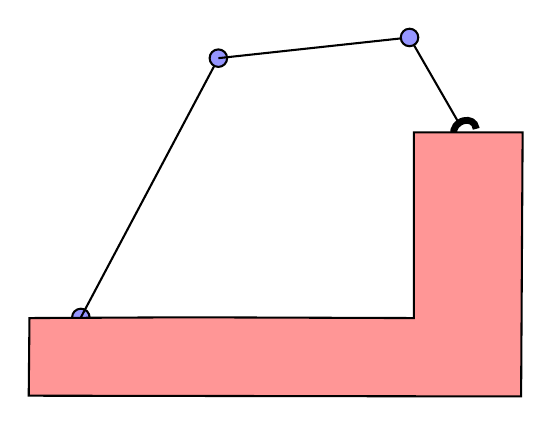
\begin{tikzpicture}[x=0.55pt,y=0.55pt,yscale=-1,xscale=1]
%uncomment if require: \path (0,300); %set diagram left start at 0, and has height of 300

%Shape: Circle [id:dp2680036705913309] 
\draw  [fill=myblue  ,fill opacity=1 ] (144.5,190.35) .. controls (144.5,187.17) and (147.07,184.6) .. (150.25,184.6) .. controls (153.43,184.6) and (156,187.17) .. (156,190.35) .. controls (156,193.53) and (153.43,196.1) .. (150.25,196.1) .. controls (147.07,196.1) and (144.5,193.53) .. (144.5,190.35) -- cycle ;
%Straight Lines [id:da511009501867824] 
\draw    (150.25,190.35) -- (240.6,20) ;
%Shape: Circle [id:dp33456176340238253] 
\draw  [fill=myblue  ,fill opacity=1 ] (234.85,20) .. controls (234.85,16.82) and (237.42,14.25) .. (240.6,14.25) .. controls (243.78,14.25) and (246.35,16.82) .. (246.35,20) .. controls (246.35,23.18) and (243.78,25.75) .. (240.6,25.75) .. controls (237.42,25.75) and (234.85,23.18) .. (234.85,20) -- cycle ;
%Straight Lines [id:da8106680503102979] 
\draw    (240.6,20) -- (366.2,6.4) ;
%Straight Lines [id:da7152287278059997] 
\draw    (399.4,64) -- (366.2,6.4) ;
%Shape: Circle [id:dp1080265764134869] 
\draw  [fill=myblue  ,fill opacity=1 ] (360.45,6.4) .. controls (360.45,3.22) and (363.02,0.65) .. (366.2,0.65) .. controls (369.38,0.65) and (371.95,3.22) .. (371.95,6.4) .. controls (371.95,9.58) and (369.38,12.15) .. (366.2,12.15) .. controls (363.02,12.15) and (360.45,9.58) .. (360.45,6.4) -- cycle ;
%Shape: Block Arc [id:dp8677516838116468] 
\draw  [fill={rgb, 255:red, 0; green, 0; blue, 0 }  ,fill opacity=1 ] (397.16,75.17) .. controls (396.21,74.66) and (395.39,73.93) .. (394.76,73.02) .. controls (392.25,69.38) and (393.66,64.05) .. (397.92,61.11) .. controls (402.18,58.16) and (407.67,58.73) .. (410.18,62.36) .. controls (410.82,63.28) and (411.2,64.3) .. (411.35,65.37) -- (408.23,66.19) .. controls (408.19,65.47) and (407.96,64.78) .. (407.55,64.18) .. controls (406.04,62) and (402.55,61.8) .. (399.74,63.74) .. controls (396.94,65.68) and (395.88,69.02) .. (397.39,71.2) .. controls (397.8,71.8) and (398.37,72.25) .. (399.02,72.54) -- cycle ;
%Shape: Polygon [id:ds12621320375323086] 
\draw  [fill=mypink  ,fill opacity=1 ] (440.5,68.75) -- (369,68.75) -- (369,190.75) -- (219.5,190.25) -- (116.5,190.75) -- (116,241.75) -- (439.5,242.25) -- cycle ;




\end{tikzpicture}

    %\caption{Caption}
    %\label{fig:my_label}
\end{figure}

\end{flushleft}
\end{frame}



\begin{frame}
\centerline{Lecture slides are available via Moodle.}
\bigskip
\centerline{You can help improve these slides at:}
\centerline{\href{https://github.com/SergeiSa/Contact-Aware-Control-Slides-Fall-2020}{github.com/SergeiSa/Contact-Aware-Control-Slides-Fall-2020}}
\bigskip
\centerline{Check Moodle for additional links, videos, textbook suggestions.}
\end{frame}

\end{document}
